\documentclass[../main.tex]{subfiles}

\begin{document}

Con esta subsección se pretenden aplicar los contenidos expuestos en apartados descritos en esta misma sección desde un punto de vista más técnico y práctico. Para ello, se ha implementado un sistema capaz de reproducir una situación lo más parecida posible a la realidad. 
\\

En primer lugar se expondrán los \hyperref[Definición de flujos de acción]{flujos de acción} disponibles mediante sus correspondientes diagramas, seguido de una \hyperref[Visión general del sistema]{visión general} del comportamiento y aspecto del mismo, concluyendo finalmente con un breve análisis sobre las \hyperref[Análisis sobre las tecnologías empleadas]{tecnologías} empleadas.
\\

% ------------------------------
% Definición de flujos de acción
% ------------------------------
\subsubsection{Definición de los flujos de acción.}\label{Definición de flujos de acción}

En el sistema intervendrán los propios \hyperref[Actores y sus funciones en el paradigma]{actores} del paradigma introducidos con anterioridad (Emisor, Titular y Verificador), a los cuales se añadirán los siguientes:

\begin{itemize}
    \item \textbf{Registro}. \\
    El Titular debe adquirir un token de control de acceso al Servicio que es expedido por este actor. Este comportamiento es típico de protocolos tipo \Gls{OpenID} y gracias a la \acrshort{SSI} se obtiene la garantía de identificar inequívocamente al usuario. 

    \item \textbf{Servicio}. \\
    Representa el objetivo final del Titular, por el cual ha requerido de sus credenciales para identificarse. Dependiendo del flujo escogido variará  el método de acceso al mismo.\\
    
\end{itemize}

Con el objetivo de facilitar la monitorización del sistema en su conjunto, se introducirá un nuevo cuasi-actor al que se denominará \textbf{main}. Como su propio nombre indica, será el ejecutor de la batería de pruebas (de ahora en adelante llamados \textbf{pasos}) y no es considerado como parte del sistema ya que no realiza ninguna función más allá de recibir y mostrar al usuario los mensajes obtenidos por el Titular. 

\newpage

\begin{enumerate}[label=\textbf{\Alph*.}]
    % --------------------------
    \item \textbf{El Titular debe pasar por el Registro para poder hacer uso del Servicio.} \\
    \begin{figure}[htbp]
        \centering
        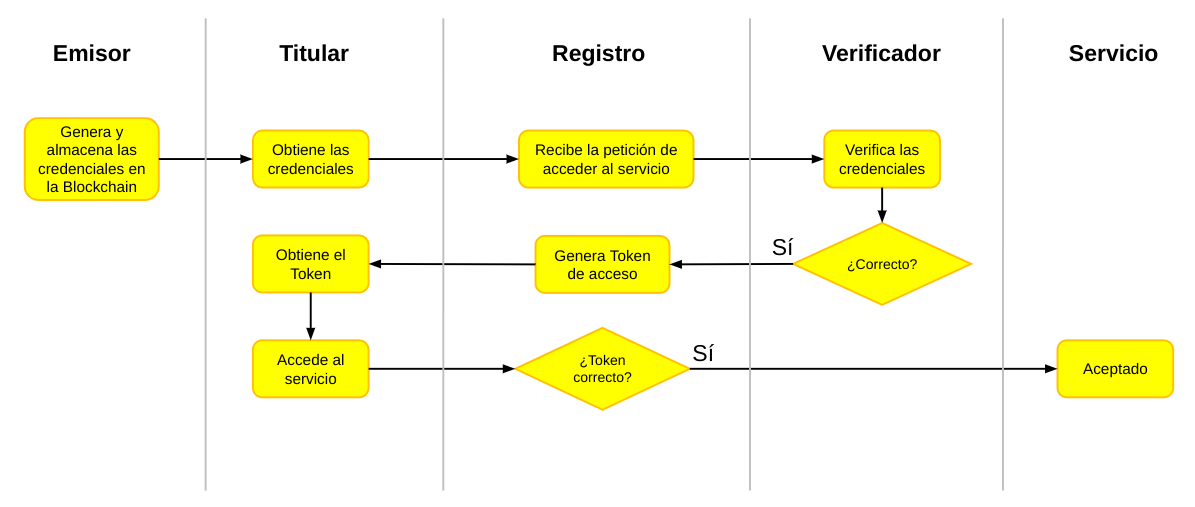
\includegraphics[width=1\linewidth]{images/PoC_A.png}
        \caption{\textit{Flujo de comunicaciones para la Prueba de Concepto A.}}
    \end{figure}

    \vspace{1cm} 

    % --------------------------
    \item \textbf{El Titular puede interactuar con el Servicio, pero solo podrá valerse de él una vez se compruebe el token proporcionado en el Registro.} \\    
    \begin{figure}[htbp]
        \centering
        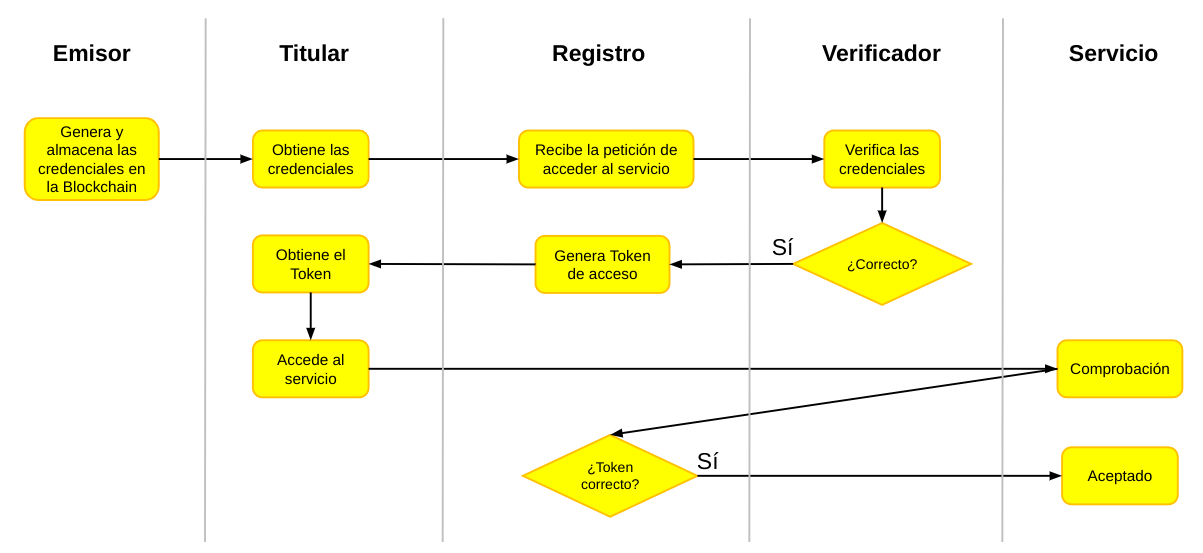
\includegraphics[width=1\linewidth]{images/PoC_B.png}
        \caption{\textit{Flujo de comunicaciones para la Prueba de Concepto B.}}
    \end{figure}

\end{enumerate}


\newpage

\noindent En términos generales, se respetará el transcurso natural de las operaciones de los actores:

\begin{enumerate}[label=\textbf{Paso \arabic*.}, leftmargin=5em]
    \item Actores involucrados: \textit{Emisor}, \textit{Titular}. El Titular pide al Emisor generar una \acrshort{VC} para poder ser identificado y guarde su \Gls{hash} en la Blockchain. 
    \item Actores involucrados: \textit{Titular}, \textit{Registro}, \textit{Verificador}. El Titular realiza una petición de acceso al Registro, el cual genera un token tras la confirmación del Verificador. 
    \item Actores involucrados: \textit{Titular}, \textit{Registro}, \textit{Servicio}. El Titular utiliza su token para autenticarse en el Registro y acceder al Servicio. También puede utilizarlo directamente en el Servicio, siendo necesaria una comprobación posterior en el Registro. 
\end{enumerate}


% --------------------------
% Visión general del sistema
% --------------------------
\subsubsection{Visión general del sistema.}\label{Visión general del sistema}
A continuación, se mostrará a grandes rasgos el funcionamiento del sistema desarrollado el cual se describirá con mayor grado de detalles técnicos en el \hyperref[Configuración de la prueba de concepto]{apéndice} de este mismo \acrshort{TFG}. 

\noindent El primer aspecto que el usuario tendrá que decidir es cuál de los flujos descritos con anterioridad seguirá, teniendo que pinchar en uno de los dos botones azules designados para ello.
\\

\begin{figure}[htbp]
    \centering
    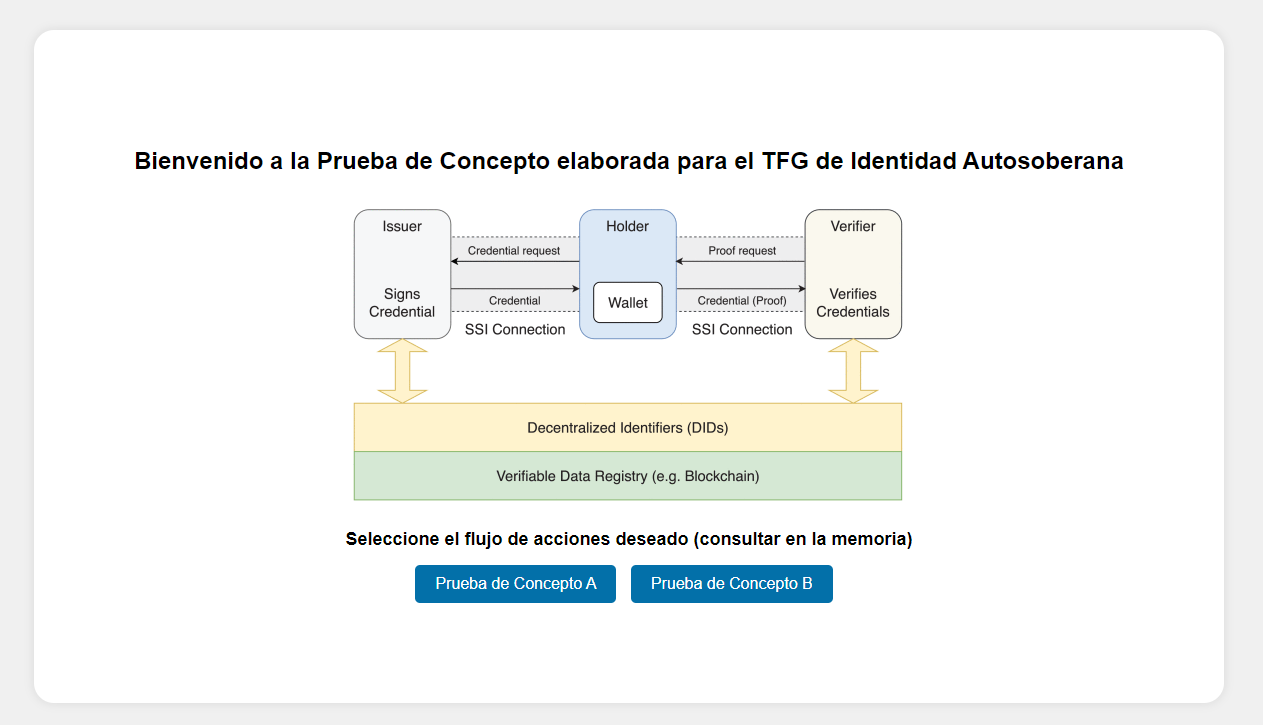
\includegraphics[width=1\linewidth]{images/design/landing.png}
    \caption{\textit{Página principal del sistema.}}
\end{figure}

\noindent Dependiendo de su elección, dispondrá de las siguientes páginas las cuales incluyen: 
\begin{itemize}
    \item Un recuadro \textcolor{gray}{gris} en el que se mostrará el estado final de las comunicaciones.
    \item Sendos botones \textcolor{blue}{azules} correspondientes a cada paso del flujo en cuestión.
    \item Un botón \textcolor{red}{rojo} para volver a la página principal de inicio y escoger otro flujo.
\end{itemize}

\begin{figure}[htbp]
    \centering
    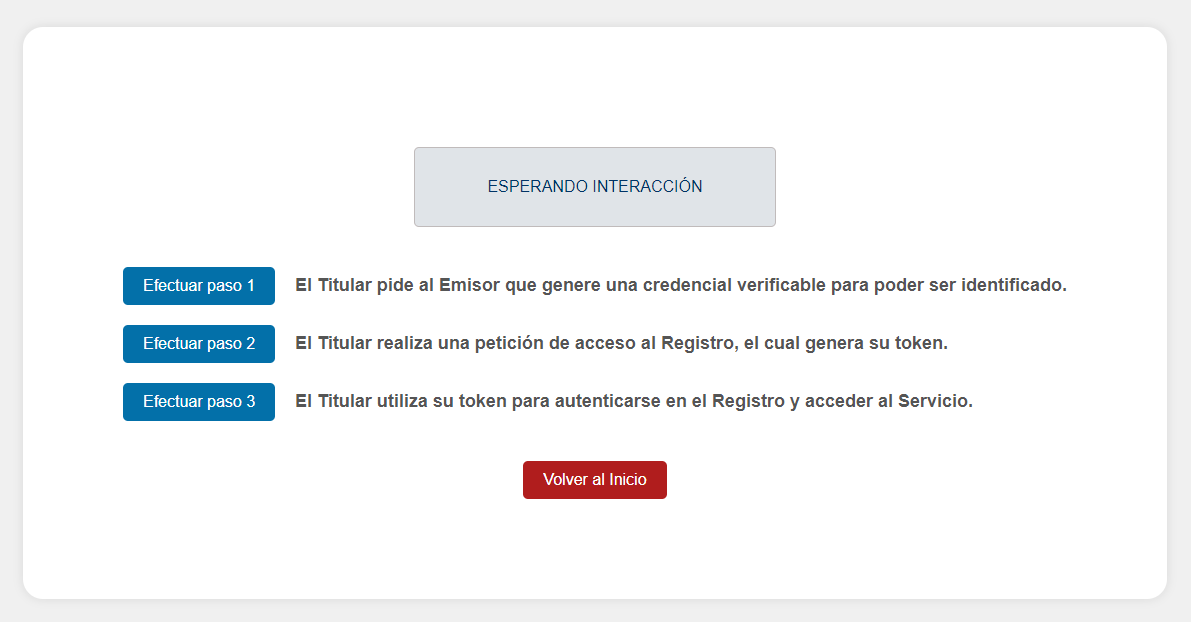
\includegraphics[width=0.9\linewidth]{images/design/PoCA.png}
    \caption{\textit{Página de la Prueba de Concepto A.}}
\end{figure}

\begin{figure}[htbp]
    \centering
    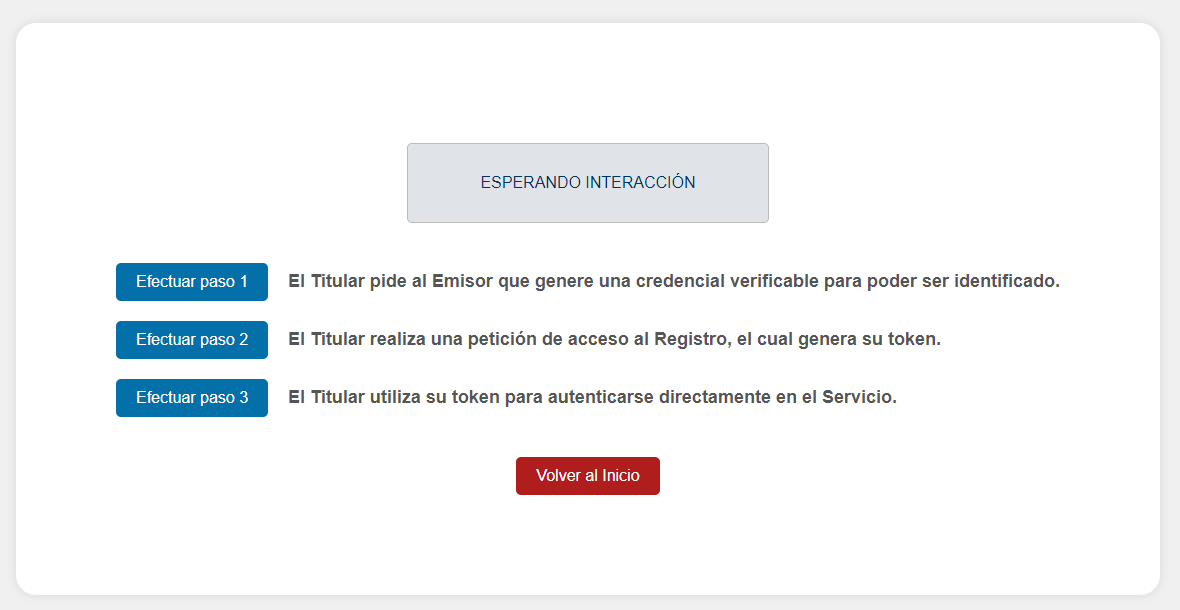
\includegraphics[width=0.9\linewidth]{images/design/PoCB.png}
    \caption{\textit{Página de la Prueba de Concepto B.}}
\end{figure}

\newpage
% ----------------------------------------
% Análisis sobre las tecnologías empleadas
% ----------------------------------------
\subsubsection{Análisis sobre las tecnologías empleadas.}\label{Análisis sobre las tecnologías empleadas}
Finalmente, se realizará una breve introducción a los medios técnicos que fueron empleados para la implementación de la prueba de concepto descrita con anterioridad. Con esto no se pretende dar una visión general de la tecnología, más bien destacar los motivos por los que fueron escogidos y la función que desempeñan en su conjunto.  
\\

\begin{itemize}

    % --------------------
    \item \textbf{Python}. \\ 
    La lógica interna del sistema estará implementada principalmente en \textit{Python} y se basará en frameworks propios como \textit{Flask} para establecer las conexiones necesarias durante las comunicaciones entre los componentes (actores) del mismo. 
    \\ 
    
    La decisión de emplear \textit{Python} se fundamenta en la simplicidad de su sintaxis y la consecuente legibilidad del código elaborado, además de la posibilidad de importar numerosas librerías relacionadas con el paradigma. Dichos aspectos, entre otros, han convertido a \textit{Python} en uno de los lenguajes de programación más utilizados de los últimos tiempos. 
    \\ 
    
    En el sistema, se conectarán los componentes con el intercambio de mensajes estructurados en formato JSON incluidos en peticiones HTTP, empleando para ello la librería Urllib (aunque pueden emplearse alternativas). Además, \textit{Flask} permite la integración de recursos propios del desarrollo web, como HTML, CSS y JavaScript, los cuales servirán para acceder al monitorizador del sistema mediante el navegador. 
    \\
    
    \begin{figure}[htbp]
        \centering
        
\includegraphics[width=0.25\linewidth]{images/technologies/python.jpg}
        \caption{\textit{Logo oficial de \textbf{Python}.}}
    \end{figure}
   
    % --------------------
    \item \textbf{Docker}. \\ 
    Uno de los requisitos indispensables del sistema es mantener los componentes aislados entre sí, ya que es necesario simular un entorno real en el que cada actor puede realizar su función en el paradigma de manera autónoma e independiente.
    \\

    Esto se conseguirá `dockerizando' individualmente cada fichero que abstrae el comportamiento de los diferentes actores, generando así un conjunto de `imágenes' que sean fáciles de `desplegar' mediante su agrupación en un `contenedor'. Además, gracias a este proceso se elimina la necesidad de tener instaladas en el dispositivo las dependencias necesarias para su correcto funcionamiento, agilizando entonces su portabilidad.
    \\
    
    \begin{figure}[htbp]
        \centering
        
\includegraphics[width=0.45\linewidth]{images/technologies/docker.png}
        \caption{\textit{Logo oficial de \textbf{Docker}.}}
    \end{figure}
  
    % --------------------
    \item \textbf{Kubernetes}. \\ 
    Aunque no sería necesario per se, es posible realizar un despliegue en \textit{Kubernetes} para la mejor orquestación en `pods' (conjunto de imágenes que conforman el contenedor) de nuestro sistema. Esta alternativa nos permite tener un mayor control sobre la gestión, escalado y exposición de los mismos, aunque suele estar pensada para entornos más complejos y de mayor envergadura que el nuestro. Cabe destacar que \textit{Kubernetes} no es un sustituto de \textit{Docker}, más bien es una extensión que amplía el alcance de las capacidades de \textit{Docker}, empleando como base los recursos generados por él.
    \\
    
    \begin{figure}[htbp]
        \centering
        
\includegraphics[width=0.45\linewidth]{images/technologies/kubernetes.png}
        \caption{\textit{Logo oficial de \textbf{Kubernetes}.}}
    \end{figure}

    \newpage
    % --------------------
    \item \textbf{PyCharm}. \\ 
    El \Gls{entorno de desarrollo} empleado para estructurar el sistema es \textit{PyCharm}, por un mero motivo de preferencia personal y al estar orientado a desarrollar código \textit{Python}. Una facilidad que ofrece ante alternativas como \textit{Visual Studio Code} es la integración nativa de herramientas de orquestación y gestión de entornos virtuales como \textit{Kubernetes}.
    \\
    
    \begin{figure}[htbp]
        \centering
        
\includegraphics[width=0.25\linewidth]{images/technologies/pycharm.jpg}
        \caption{\textit{Logo oficial de \textbf{PyCharm}.}}
    \end{figure}
    
    % --------------------
    \item \textbf{Besu Hyperledger}. \\ 
    En el apartado técnico de la Blockchain, se obtendrá desde Docker Hub la imagen del cliente de Ethereum, implementado en JAVA y de código abierto \textit{Besu Hyperledger}. 
    
    La característica clave por la que se ha escogido esta solución entre otras similares es lo adecuada que resulta para el sistema, ya que crea una red privada dentro un contenedor y permite configurar aspectos como el establecimiento de las comunicaciones con HTTP.

    Los actores interactuarán con la red mediante la libreria Web3 para realizar las pertinentes transacciones acordes a las necesidades de la \acrshort{SSI}, disponiendo de funciones tras el despliegue del contrato elaborado en \textit{Solidity} para ello. Ejemplo de esto es el almacenamiento de los \acrshort{DID}s y el \Gls{hash} de las \acrshort{VC} creados mediante la librería DIDKit de \textit{Python}.
    \\ 

    \begin{figure}[htbp]
        \centering
        
\includegraphics[width=0.5\linewidth]{images/technologies/besu.png}
        \caption{\textit{Logo oficial de \textbf{Besu Hyperledger}.}}
    \end{figure}

\end{itemize}

\end{document}